% This is a basic Math Paper

\documentclass[11pt]{article}

% Preamble

\usepackage[margin=1in]{geometry}
\usepackage{amsfonts, amsmath, amssymb}
\usepackage{fancyhdr, float, graphicx}
\usepackage[utf8]{inputenc} % Required for inputting international characters
\usepackage[T1]{fontenc} % Output font encoding for international characters
\usepackage{fouriernc} % Use the New Century Schoolbook font
\usepackage[nottoc, notlot, notlof]{tocbibind}
\usepackage{url}

% Header and Footer
\pagestyle{fancy}
\fancyhead{}
\fancyfoot{}
\fancyhead[L]{\textit{\Large{HDPC Group Activity}}}
%\fancyhead[R]{\textit{something}}
\fancyfoot[C]{\thepage}
\renewcommand{\footrulewidth}{1pt}



% Other Doc Editing
% \parindent 0ex
%\renewcommand{\baselinestretch}{1.5}

\begin{document}
	
	\begin{titlepage} 
		\centering 
		
		%---------------------------NAMES-------------------------------
		
		\huge\textsc{
			MIT World Peace University
		}\\
	
		\vspace{0.75\baselineskip} % space after Uni Name
		
		\LARGE{
			Human Dynamics and Peace in Communications\\
			First Year B. Tech, Trimester 3\\
			Academic Year 2021-22
		}
		
		\vfill % space after Sub Name
		
		%--------------------------TITLE-------------------------------
		
		\rule{\textwidth}{1.6pt}\vspace*{-\baselineskip}\vspace*{2pt}
		\rule{\textwidth}{0.6pt}
		\vspace{0.75\baselineskip} % Whitespace above the title
		
		
		
		\huge{\textsc{
				Interaction with the Elderly
			}} \\
		
		
		
		\vspace{0.5\baselineskip} % Whitespace below the title
		\rule{\textwidth}{0.6pt}\vspace*{-\baselineskip}\vspace*{2.8pt}
		\rule{\textwidth}{1.6pt}
		
		\vspace{1\baselineskip} % Whitespace after the title block

		%--------------------------SUBTITLE --------------------------	
			
		\LARGE\textsc{
			Group Activity
		} % Subtitle or further description
		\vfill
		
		%--------------------------AUTHOR-------------------------------
		
		Prepared By
		\vspace{0.5\baselineskip} % Whitespace before the editors
		
		\Large{
			109054. Krishnaraj Thadesar\\
			109056. Tirth Thesiya\\
			109050. Atharva Tanavade\\
			109052. Arnav Tavergeri\\
			109021. Vedant Shirode\\
			109071. Pranav Walvekar\\
			\vspace{1cm}
			Division 9 Batch I3
		}
		
		
		\vspace{0.5\baselineskip} % Whitespace below the editor list
		\today

	\end{titlepage}

\clearpage

\noindent
\Large{\textbf{A Brief Summary of the Interactions}}\\

All the members of the team interacted with several elderly people, and asked them some basic questions. We introduced ourselves as students
from MIT WPU, in search of their views on some pressing questions. A breif summary of all the interaction that took place between all the 
students and the eldery is given here. \\

\noindent
\textbf{Purpose of this Activity}\\

\textit{"The purpose of this experiment according to us is to connect this years generation with the old generation, as we all know in todays
 busy world no one gets time for anyone as everyone is busy in their own life but this should not be
the case as our grandparents who are growing older day by day they have no one to connect to 
and share their thoughts and also most of them can't be much active due to their health and we as their grandchildren should be always connected with them as they have helped us so much we cant even express in words and we should be 
caring, loving and help them do their chores and just be in their position and realize how they live their life."}\\


\noindent
\textbf{Q1. How do you look at today's Youth?}\\

\textit{"Today's youth is just like any other youth, but due to internet and the fact that their exposure to the entire world
is so much more than what we had before, is what makes them different. I do not think that they are rude, or arrogant, because all 
teenagers have been arrogant in the past, and this generation is no different. But with the new technologies that are emerging every day, 
they are forgetting the importance of people, and offline interactions, that used to exist in our times. People are the most important aspect
of our lives in my opinion, and sooner or later, I think that this generation will also realize that."}\\

\textbf{Q2. What is your opinion about the current generation gap?}\\

\textit{"Generation gap is going to be prevalent wherever you go because the ideals of the younger generation and older generation always differ in some way which creates a rift between the two generations.
Though, in today's time, the generation gap is smaller than it used to be, around 10-20 years ago.
This is due to the fact that every person young and old has access to technology, which has become extremely user friendly.
This helps in the older generation connecting with the younger generation easily, as they are up to date with trends, as well as the rapidly changing world around them.
The older generation are also slowly rising up from their conservative mindsets and accepting the changes."}\\

\textbf{Q3. What Advice would you like to give to today's Youth}

\textit{"This generation must learn to understand that the most important thing in life is family. Everything that we earn in life, we will 
have to spend someday, the only thing that will always stay with you is your family, and that is something that I have also realized after
a long time."}\\

\textbf{Q4. What are some of the challenges that you face? They may be concered with your health, society, Finance, Culture etc.}\\

\textit{"As a senior citizen, there are certain things that pose me some difficulty every now and then, while some are ones I face every day. 
Health wise everything is what you would expect from a person in their Sixtees. So no surprises there, Financially, I have been lucky enough to 
save for myself, and my son takes good care of me. But the culture is what challenges me the most. I find the culture of today wildly different
from what it used to be long back. Socially, things are better now than they used to be before. Our country has only advanced forward in the past few years. 
And things have been getting better and better for senior citizens and medical technology advances every day." }\\

\textbf{Q5. How is your Rapport with your Grandchildren?}\\

\textit{"(Laughs)... Well, as you can see my grandson is sitting right here listening to everything. That should tell you how things are. But to answer your question, 
The best part of a senior citizens life are his or her grandchildren. They make you forget all the problems that you have, and make you realize that they are the most 
important things in the world. Even as they grow older, and enter into their teenage, they may end up fighting with their parents, but it is very very rare that they ever
get into a fight with their grandparents. Sure our thoughts might differ on many subjects, but that has never come in the way of our love and affection. At this point it has become
something that we do involuntarily."}\\

\centering
\Large{\textbf{Pictures taken by our group}}

\begin{figure}[H]
	\centering
	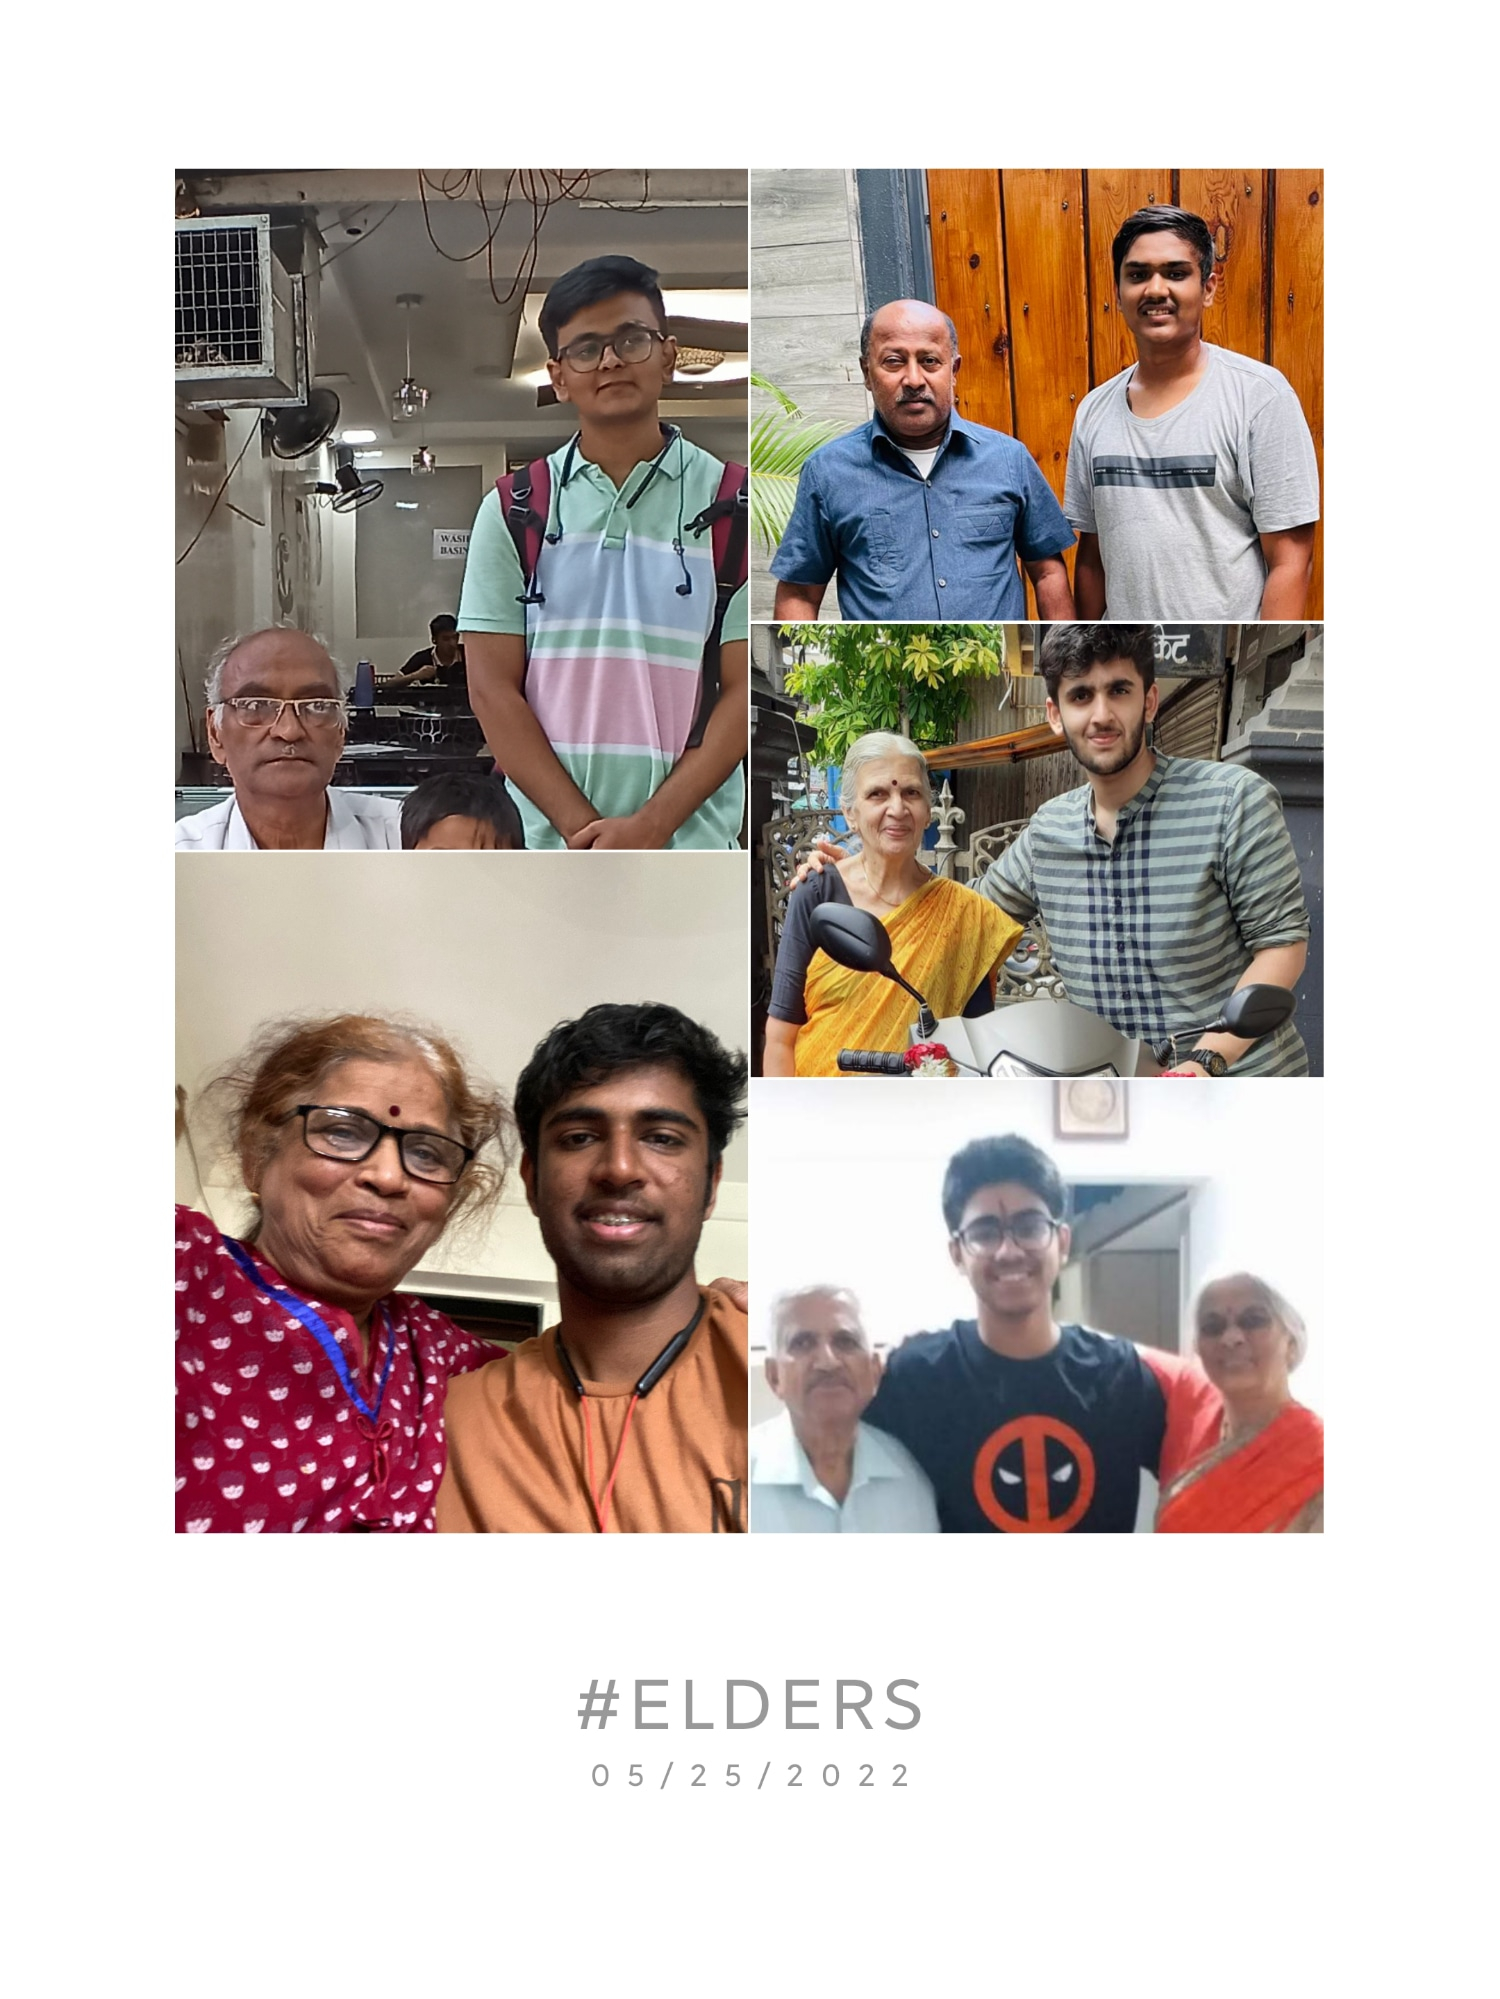
\includegraphics[scale=0.25]{WhatsApp Image 2022-05-25 at 00.32.11 (1).jpeg}
	\label{it}
\end{figure}

\end{document}